\clearpage
\subsection*{保存房间里的反射光}

浴室的点光源固定在柜台与窗边。把相机靠近洗手盆，盆沿落在了新的像素上，照到它的反射光仍来自原来那间屋子。探针记录的是房间中固定位置的光量，因而可以在布光完成后把它们算好，保存到场景旁边。这一步叫作烘焙。

在 Vulkan 编辑器打开并保存场景，在「实时效果」中选择 DDGI，再展开渲染设置的「质量与参数」。点「烘焙探针」，每个探针朝六个方向取样，每个方向发出 64 条射线。每轮共 $12\times6\times7\times6\times64=193\,536$ 条，射线碰到表面时还要查点光源的遮挡。勾选默认的「多次漫反射」会依次算四轮，让前一轮照亮的表面继续反光，共 774\,144 条探针射线；关闭时只算第一轮。完成后面板显示「已烘焙」。

\begin{center}
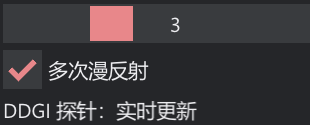
\includegraphics[width=.43\linewidth]{figures/probe-controls.png}\hspace{.04\linewidth}
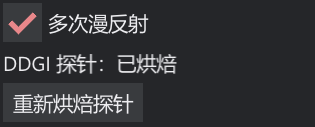
\includegraphics[width=.43\linewidth]{../../../output/profiling/point-materials/bathroom-reopened.png}\\[-1pt]
{\small 浴室实拍。左图记录早期的实时模式；右图在点光源更新后重新烘焙，退出并重开后显示「已烘焙」。}
\end{center}

每个方向留下两个四维向量。第一组的前三项是红、绿、蓝的间接光，第二组的前两项是命中距离及其平方的平均。沿用着色器的存法，两组共占 32 字节。整间房有 $12\times6\times7\times6=3\,024$ 组方向记录，合计 96\,768 字节，加上文件头共 96\,792 字节。浴室的文件名是 \texttt{RTXGI-Bathroom.redflag.rfprobes}。

重新打开场景时，程序把模型三角形、材质、贴图和点光源与烘焙时的记录核对。相符的探针直接传回显卡。接着照常为眼前的像素寻找附近的探针，移动相机、改变面板大小都可以继续用这份数据。把柜门换成另一种颜色或移走窗边灯，旧数据就失去了依据。面板会切回「实时更新」，此时再烘焙一次即可。

\noindent{\small\color{quiet}C++ 接口调用示例\quad\href{run:../../Redflag/src/Redflag/Renderer/GI/GlobalIllumination.cpp}{\texttt{GlobalIllumination.cpp}}}\par\nopagebreak
\begin{lstlisting}[escapeinside={(*@}{@*)}]
gi.SetLights(sceneLights);
gi.BakeProbes(file);  (*@{\footnotesize\color{quiet}// 把房间各处收到的反射光写入场景旁的文件。}@*)

(*@{\footnotesize\color{quiet}// 下次打开后，先按场景恢复模型与点光源，再尝试读回上次的结果。}@*)
bool ready = gi.LoadProbes(file);
gi.Render(GIMethod::DDGI);  (*@{\footnotesize\color{quiet}// 如果上次的光照已过期，这一帧会重新计算探针。}@*)
\end{lstlisting}

在 Sponza 固定机位，先从一个进程输出 $160\times90$ 的间接光，再退出并用第二个进程加载文件。两张图全部 14\,400 个 HDR 像素逐字节相同。浴室还多试了一步，烘焙后按 Ctrl+S 再退出。场景文件把三盏灯按相反顺序写回去，重新打开仍显示「已烘焙」。点光源排列顺序可以改变，位置、强度、颜色和影响半径都参与核对。RenderDoc 里保留了给表面插值的计算，省掉了更新探针的一遍。\href{run:Redflag-Rendering-Performance.pdf}{《渲染性能实测》}
